
\chapter{Efficient KD-Tree For Ray-Tracing}
\setcounter{figure}{1}      % reset the figure counter
\label{ch:effiecient_kd-tree}

\section{KD-Tree Construction Algorithm} 
The general kd-tree construction algorithm has been presented in the previous text, in this section, more advanced techniques adopted on the construction of kd-tree will be discussed in depth.

\subsection{Surface Area Heuristic}

In the algorithm \ref{algo:kd-tree_construction}, a recursive construction of kd-tree in top-down fashion has been presented, essentially all kd-tree construction algorithm follow the same scheme. The key operation in the construction of kd-tree is to effectively picking a split plane in every subdivision. There are several best known methods for positioning the splitting plane in the kd-tree:

\begin{comment} 
\begin{figure}[htp] 
    \centering 
    \fbox{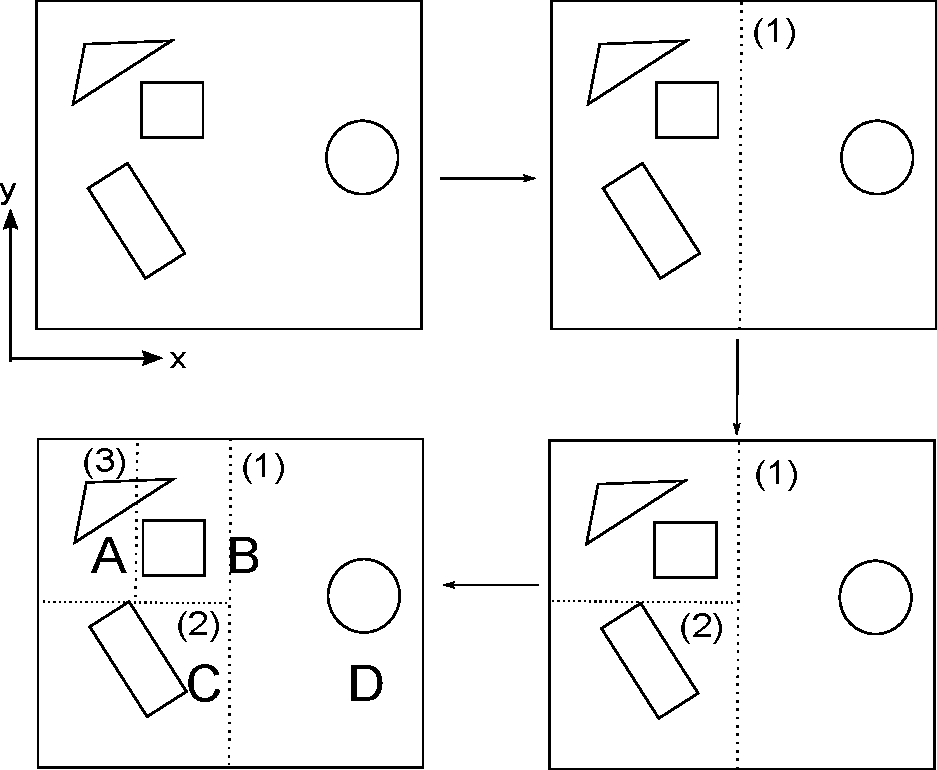
\includegraphics[width=\linewidth]{figKDTreeSubdivideSpatialMid.pdf}} 
    \renewcommand{\thefigure}{\thechapter.\arabic{figure}}
    \caption[The scene with the spatial median subdivision]{\emph{ The scene with the spatial median subdivision}}
    \label{fig:kd-tree_subdivide_spatial_mid}
\end{figure}
\end{comment}

% what is SAH
In \cite{havran2000}, Vlastimil Havran introduced ``surface area heuristic'' (SAH), which provides a well-grounded cost model that estimates the average cost of traversing an arbitrary ray through the kd-tree. The estimated cost is used to determine which split plane among a number of split candidates should be chosen in order to lead to a more efficient acceleration structure for ray-primitives testing. Most of the best current acceleration structures' building algorithms are based on SAH cost model. 

The SAH cost model provides an estimation of the computational expense of performing ray intersection tests, including the time spent traversing nodes of the tree and the time spent on ray-primitive intersection test for a subdivision of primitives. The goal for the kd-tree construction algorithm to follow is to minimize the total cost, particularly for a greedy algorithm like algorithm \ref{algo:kd-tree_construction}, the goal is to minimize the cost for each subdivision step.

For each subdivision step, we have to decide whether to make the current region a leaf node with all of the overlapping primitives attached or refine the region to create two subregions. In the first case, any ray that passes through this region will be tested against all of the primitives leading to a cost of 
        $\displaystyle\sum\limits_{i=1}^N C_{isect}(i)$

Where N is the number of primitives and \(C_{isect}(i)\) is the cost of computing the intersection between the ray and the \(i\)th primitive. 

For the other case which is to split the region, the cost can be modeled with the following equation:

\begin{equation} 
        \label{eq:CostOneStep}
        C(A, B) = C_{trav} + p_{A} \cdot \sum\limits_{i=1}^{N_{A}} C_{isect}(a_{i}) + p_{B} \cdot \sum\limits_{i=1}^{N_{B}} C_{isect}(b_{i})
\end{equation}

Where the \(C_{trav}\) is the cost of traversing the interior node, \(p_{A}\) and \(p_{B}\) are the probabilities of the ray passing through each of the child nodes. \(a_{i}\) and \(b_{i}\) are the primitives attached on the two children nodes, and \(N_{A}\) and \(N_{B}\) are the number of the primitives overlapping with of the subregions respectively. 

The probabilities \(p_{A}\) and \(p_{B}\) can be computed using the ideas from geometric probability. A convex volume A contained in another convex volume B, the conditional probability that a random ray passing through B will also pass through A is the ratio of their surface areas, \(s_{a}\) and \(s_{b}\): 
\begin{equation} 
        p(A|B) = \frac{s_{A}}{s_{B}} 
\end{equation}

\subsection{KD-Tree Construction With SAH} 
As described in the chapter \ref{ch:background}, the kd-tree is built with a recursive top-down algorithm. At each step, we have an axis-aligned region of space and a set of primitives that overlap the region. Either the region is split into two subregions and turned into an interior node, or a leaf node is created with the overlapping primitives, terminating the recursion.  
% why is the SAH-based kd-tree beneficial for the ray-tracing
The strategy of choosing the split plane in the kd-tree construction process may have considerable impact on the performance of ray-tracer. An \mynaive approach is to place the split plane at the middle of region along certain axis splitting each node in half at each level and generating a balanced binary tree. Similar to the binary search tree, this approach is beneficial when the goal is to quickly figure out in which leaf node a certain point locates. However, in addition to quickly query the geometric primitive hit by the ray, the goal of kd-tree traversal is to find the closest intersection point. With the strategy of picking the spatial middle point as the split plane, it is likely to create the leaf nodes which contain lots of geometr as the distribution of geometry is not taken into account. The disadvantage of this approach is that whenever a ray traverses through a leaf node, it has to test for intersection with all of the primitives even there is no chance they could intersect. To minimize the redundant intersection tests, the distribution of geometry has to be somehow encoded into the kd-tree built from a certain scene to provide heuristic information for the ray tracer in kd-tree traversal stage. It is optimal to maximize the space of the leaf node which contains little geometry and minimize the space that contains more geometry. Figure \ref{fig:kd-tree_subdivide_spatial_mid_vs_sah} shows the different effect when traversing the tree built by two different approaches. 

\begin{figure}[htp] 
    \centering 
    \fbox{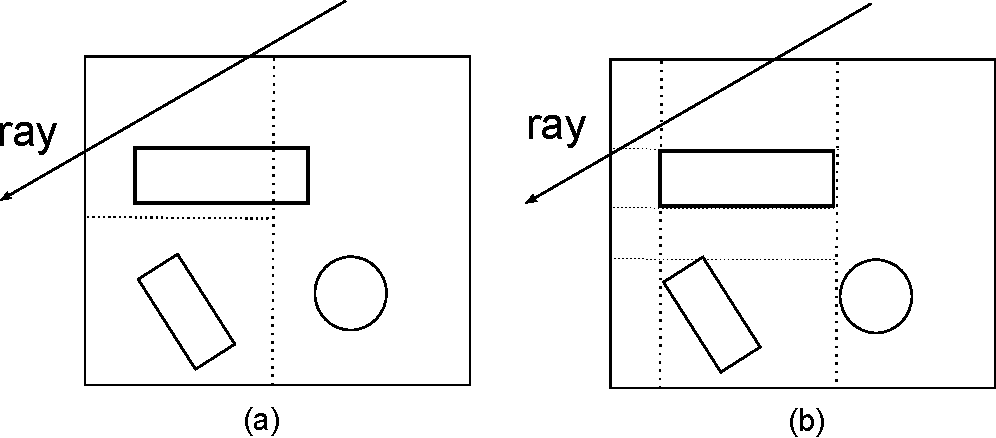
\includegraphics[scale=0.8]{figKDTreeSubdivideSpatialMidVsSAH.pdf}} 
    \renewcommand{\thefigure}{\thechapter.\arabic{figure}}
    \caption[Spatial median split and SAH-based split]{(a) The scene is subdivided using the spatial middle point and the created leaf nodes will cause redundant intersection tests. (b) The scene is subdivided based on the SAH cost model resulting a higher quality kd-tree. When a ray traverse through the kd-tree, it can quickly skip those leaf nodes without performing intersection tests since the empty region is isolated from the region that contains more geometry.}
    \label{fig:kd-tree_subdivide_spatial_mid_vs_sah}
\end{figure}

% SAH-based kd-tree construction 
With the definition of the SAH cost model, we can easily adopt the SAH in the kd-tree construction algorithm. As shown in the algorithm \ref{algo:kd-tree_construction_sah}. 

The termination criteria of the SAH-based algorithm is more stable when to stop subdivisions. As the cost of a leaf node can be modeled as \(C_{leaf} = K_{isect}\lvert T \rvert\), the subdivision will be terminated when the further split of this leaf node has higher cost than not splitting at all. 

The ``FindSplitPlaneSAH'' function takes the list of triangles \(T\), the voxel that to be split \(V\) and an axis \(k\) as the input parameters, outputs the split with the minimum cost. However, this process is not trivial compares to the spatial median splitting which only costs \mycomplexityconst. To calculate the cost for each split candidates, we have to determine the number of primitives of both left and right child \(N_{L}\) and \(N_{R}\). This can be done by classifying the triangle list which cost \mycomplexityn. Therefore the overall complexity for finding the optimal split algorithm is \mycomplexitysqrtn. 


\SetAlFnt{\small}
\begin{algorithm}[H]
        \SetAlgooLined
        \SetKwData{true}{\(true\)}
        \SetKwData{false}{\(false\)}

        \SetKwData{tri}{\(t\)}
        \SetKwData{triangleList}{\(T\)}
        \SetKwData{triangleListLeft}{\(T_{L}\)} 
        \SetKwData{triangleListRight}{\(T_{R}\)}
        \SetKwData{triangleListLeftNum}{\(\lvert\)\triangleListLeft\(\rvert\)}
        \SetKwData{triangleListRightNum}{\(\lvert\)\triangleListRight\(\rvert\)}

        \SetKwData{voxel}{\(V\)}
        \SetKwData{voxelLeft}{\(V_{L}\)}
        \SetKwData{voxelRight}{\(V_{R}\)}
        \SetKwData{currentNode}{\(node\)}
        \SetKwData{currentBox}{\(box\)} 
        
        \SetKwData{splitPlane}{\(p\)}
        \SetKwData{splitPlaneBest}{\(p_{best}\)}
        \SetKwData{splitPlaneCan}{ \{ \(p_0, p_1, \dots\) \} }
        \SetKwData{splitPlaneList}{\(P\)}
        
        \SetKwData{axis}{\(k\)}
        
        \SetKwData{cost}{\(C\)}
        \SetKwData{costMin}{\(C_{min}\)}

        \SetKwFunction{CalcBounds}{\ProcNameSty{CalcBounds}}
        \SetKwFunction{CalcBoundEdge}{\ProcNameSty{CalcBoundEdge}}
        \SetKwFunction{FindSplitPlaneSAH}{\ProcNameSty{FindSplitPlaneSAH}}
        \SetKwFunction{CalcSplitCandidates}{\ProcNameSty{CalcSplitCandidates}}
        \SetKwFunction{ClassifyTriangles}{\ProcNameSty{ClassifyTriangles}}
        \SetKwFunction{SAHCost}{\ProcNameSty{SAHCost}}
        \SetKwFunction{Terminate}{\ProcNameSty{Terminate}}
        
        \myfunc \ClassifyTriangles{\triangleList, \voxelLeft, \voxelRight, \splitPlane} \Return (\triangleListLeft, \triangleListRight) \newline 
        \Begin {
                \triangleListLeft = \triangleListRight = \(\phi\)\;             
                \ForAll {\tri \(\in\) \triangleList} {
                        \If {\tri overlaps with \voxelLeft} {append \tri to \triangleListLeft\;}
                        \If {\tri overlaps with \voxelRight} {append \tri to \triangleListRight\;}
                }
        }
        
        \myalgblankline
        
        \myfunc \FindSplitPlaneSAH{\triangleList, \voxel, \axis} \Return \splitPlaneBest \newline
        \Begin {
                \ForAll{\tri \(\in\) \triangleList} {
                        \splitPlane = \CalcBoundEdge{\CalcBounds{\tri}, \axis}\;
                        Append \splitPlane to split plane list \splitPlaneList\; 
                }
                \ForAll{\splitPlane \(\in\) \splitPlaneList} {
                        (\voxelLeft, \voxelRight) = split \voxel with \splitPlane\; 
                        (\triangleListLeft, \triangleListRight) = \ClassifyTriangles{\triangleList, \voxelLeft, \voxelRight, \splitPlane}\;
                        \cost = \SAHCost{V, \splitPlane, \triangleListLeftNum, \triangleListRightNum}\;
                        \If {\cost < \costMin} {
                                (\costMin, \splitPlaneBest) = (\cost, \splitPlane)\;
                        }
                }
        }
        \caption{Find the optimal split plane based on SAH}
        \label{algo:kd-tree_construction_sah}
\end{algorithm}

\subsubsection{Fast KD-tree Construction in \mycomplexitynlogn} 
It is easy to observe that the algorithm \ref{algo:kd-tree_construction_sah} is inefficient mainly due to the computation of the SAH cost for each split candidate requires the \(N_{L}\) and \(N_{R}\) which again triggers an iteration over the triangle list. In \cite{wh2006}, Wald and Havran introduced a fast SAH-based kd-tree construction algorithm whose time complexity is \mycomplexitynlogn. The improved algorithm takes the advantage of the increment of the split plane position, as the split plane ``sweeping'' over the split candidates,  the \mynumtrileft and \mynumtriright can be updated using a incremental scheme. Consider a split plane \mysplitplane in an axis \mydimension and its position is denoted as \mysplitplanepos, there is a certain number of triangles lying on the left, right side of it, which is also can be called as the number of end, starting planes respectively. Let us denote the number of starting triangles for the split plane \mysplitplane as \mynumtristartp, the number of end triangles \mynumtriendp.   

Let us consider \(n\) split planes candidates \{ \mysplitplanen{0} \}, along one fixed axis \mydimension, and assume that all the planes are sorted in ascending order. For the first split plane candidate \mysplitplanen{0} which has the minimum coordinates value, there will be no triangle on the left, all the triangles are lying on the right side of it. 

\begin{displaymath} 
    N_{L}^{(0)} = 0 \qquad N_{R}{(0)} = N
\end{displaymath} 

As the split plane ``sweeping'' from split plane \mysplitplanen{i-1} to \mysplitplanen{i}, the \mynumtrileft and \mynumtriright will change as follows: 
\begin{enumerate} 
    \item The triangles started at \mysplitplanen{i-1} will intersect with left voxel \myleftchildbox. 
    \item The triangles ended at \mysplitplanen{i} will no long intersect with right voxel \myrightchildbox 
\end{enumerate}

Therefore the \mynumtrileft and \mynumtriright can be updated incrementally using the following equations: 
\begin{equation}
        N_{L}^{i} = N_{L}^{i-1} + p^{+}
        N_{R}^{i} = N_{R}^{i-1} - p^{-}
    \label{eq:SweepUpdate}
\end{equation}

Follow this updating rule, all the \mynumtrileft and \mynumtriright of all the split planes candidates can be computed incrementally by iterating over the all the possible split position \mysplitplanen{i}. Firstly, we need to fix a dimension \mydimension, for this \mydimension, we go through all the triangles \mytriangle and generate the split candidates associated with \mytriangle, for each candidate, an ``event'' will be generated and stored. The ``event'', \myevent = (\myeventt, \myeventp, \myeventk, \myeventtype), is actually defined as a data structure which contains four data fields: a reference to the triangle whose bounding box's face defines the split candidate, the coordinate value of split position and the event type. The reference to \mytriangle can be simply an index of it, denoted as \myeventt, the plane position is a float-point value, denoted as \myeventp, the dimension \mydimension, and event type, \myeventtype, is an enumeration of several flags to indicate the relation between the triangle referenced in this event and the split plane this event corresponds to, start event and end event. According to the definition, a start event always corresponds to a split position at minimum face of the triangle's bounding box, while end event will be generated by a split plane at the position of the maximum face. Three lists of events against all axises will be generated by iterating over all the triangles, and will be eventually merged into one list \myeventlist\ in an interleaved fashion respect to the dimension, this obviously requires the event structure to have an tag to indicate which axis the event corresponds to. Secondly, each of the list of consecutive events for the same axis needs to be sorted, and the comparison of two events \(e_{a}\) and \(e_{b}\) is shown as equation \ref{eq:EventCompare}. For those events with different positions, they will be sorted by ascending the coordinate values, for those events with same positions, they will be sorted by comparing the event type, that is, the end event will precede the start event. Suppose there are two adjacent triangles which share one vertex, only one split plane candidate will be generated at the vertex, while there will be two events to be stored, one end event references the triangle that is ``before'' the plane, and one start event references the triangle that is ``beyond'' the plane. So by counting the start and end events, the \mynumtrileft and \mynumtriright can be easily determined regarding a certain plane.

% Event Comparison
\begin{equation} 
    e_{a} < e_{b} = \left\{ 
        \begin{array}{ll}
            true & (a_{p,k} < b_{p,k}) \vee ( (a_{p,k} = b_{p,k}) \wedge (a_{type} < b_{type}) ) \\
            false & otherwise
        \end{array} \right.
        \label{eq:EventCompare}   
\end{equation} 

To compute the \mynumtrileft and \mynumtriright for each split plane candidates \mysplitplanen{i} using the sorted event list to find the best one, we consider all dimensions in one loop, for each dimension, a separate \mynumtrileftk{k}, \mynumtrirightk{k}\ needs to be stored. For each dimension, we perform the ``sweeping'' using the above incremental updating scheme. We firstly consider the sequence of the \mysplitplanen{i}-related events, count the end and start events to determine the number of start and end triangles \mynumtristartip{i} and \mynumtriendip{i}. Then the \mynumtrileft and \mynumtriright for the split planes can be maintained and updated by applying the update equations. Once the \mynumtrileft, \mynumtriright are determined, the SAH cost is readily to compute and we can find the best split plane by choosing the one with minimum cost. The algorithm is shown as follows: 

\SetAlFnt{\small}
\begin{algorithm}[H]
    
    \SetKwData{vari}{i}
    \SetKwFunction{FindBestPlane}               {FindBestPlane}
    \SetKwFunction{SplitCandidates}             {SplitCandidates}
    \SetKwFunction{SAHCost}                     {SAHCost}
    \SetKwFunction{SAH}                         {SAH}
    \SetKwFunction{SplitBox}                    {SplitBox}
    
    \textbf{pre:} E has been sorted.   
    \myfunc \FindBestPlane{\myeventlistk{x,y,z}, \myvoxel, \mynumtri} \Return \mybestsplitplane\\
    \Begin {
        (\mycostmin,\mysplitplane) = (\myinfty,\myemptyset)\; 
        \ForAll {\mydimension\ in \{x, y, z\}} {
            \{start: all triangles are right side only for each k\}\\ 
            \mynumtrileftk{k} = 0, \mynumtrirightk{k} = \mynumtri\;  
            \For {$i \leftarrow 0$ \KwTo \mynumeventlist} {
                % get the plane in current k
                \mysplitplane = (\myeventlistpi{$i$}, \myeventlistki{$i$})\;
                \mynumtristartp = \mynumtriendp = 0\;
                \{iterate over all plane candidates.\}\\
                \While{$i$ \(<\) \mynumeventlist\ \(\wedge\) \mysplitplanek = \myeventlistki{$i$} \(\wedge\) \mysplitplanep = \myeventlistppi{$i$} \(\wedge\) \myeventlistti{$i$} = \myeventtypeend} { 
                    inc \mynumtriendp\;
                    inc $i$;
                }
                
                \While{$i$ \(<\) \mynumeventlist\ \(\wedge\) \mysplitplanek = \myeventlistki{$i$} \(\wedge\) \mysplitplanep = \myeventlistppi{$i$} \(\wedge\) \myeventlistti{$i$} = \myeventtypestart} {
                    inc \mynumtristartp\;
                    inc $i$\;
                }
                \mynumtrirightk{k} -= \mynumtriendp\; 
                \mycostp = \SAH{\mysplitplane,\myvoxel,\mynumtrileftk{k},\mynumtrirightk{k}}\;
                \If {\mycostp\ \(<\) \mycostmin} {
                    (\mycostmin,\mysplitplane) = (\mycostp,\mysplitplane)\;
                } 
                \mynumtrileftk{k} += \mynumtristartp\;     
            }
        }  
        \Return \mycostmin\; 
    } 
    \caption{The \mycomplexityn\ algorithm of finding the best SAH split plane}
    \label{algo:FindBestPlaneON} 
\end{algorithm}

After finding the best split plane \mybestsplitplane, classifying the triangle list into two sub-lists is another important step in one recursion step. Since the best split in current recursion is found using a sorted events list, we have to find a way to compute two sub-lists of events \myeventlistleft and \myeventlistright, and more importantly, to maintain the ascending order of them so that they can become inputs for the following recursion step without performing any sorting. As the input event list \myeventlist is sorted, and the best split plane \mybestsplitplane\ has been found, if an event is of end type and its position is less than the \mybestsplitplane, the triangle this event references must be in the left sub-list of triangle \mylefttrilist, symmetrically, the triangle referenced in a start event with a greater position than the \mybestsplitplane must belongs to the \myrighttrilist. The remaining triangles should be counted in both \mylefttrilist and \myrighttrilist. The triangle classification algorithm is shown as following: 

\SetAlFnt{\small}
\begin{algorithm}[H]
    \SetKwFunction{ClassifyTriangles}           {ClassifyTriangles}
    \myfunc \ClassifyTriangles{\mytrilist,\myeventlist,\mybestsplitplane} 
        \Return \mylefttrilist,\myrighttrilist,\myeventlistleft,\myeventlistright\\ 
    \Begin {
        \ForAll{\myevent\ \myopin\ \myeventlist} {
            \If {\myeventtype=\myeventtypestart\  
                    \myopand\ \myeventk=\mybestsplitplanek\  
                    \myopand\ \myeventp\myopless\mybestsplitplanep} {
                 
                    set \mytriflagsarray{\myeventt}.\mytriflagleft\;
                  
                } 
           \If {\myeventtype=\myeventtypeend\ 
                    \myopand\ \myeventk=\mybestsplitplanek\ 
                    \myopand\ \myeventp\myopgreater\mybestsplitplanep} {
                    
                     set \mytriflagsarray{\myeventt}.\mytriflagright\;
                 }
        } % End of ForAll event
        \ForAll {\mytriangle\ \myopin\ \mytrilist} {
            \If {\mytriflagsarray{\mytriangle}.\mytriflagleft is set} {
                \mylefttrilist\ appends \mytriangle\; 
            }
            \If {\mytriflagsarray{\mytriangle}.\mytriflagright is set} {
                \myrighttrilist\ appends \mytriangle\; 
            }
        } % End of \ForAll triangles
        
        \ForAll {\mydimension\ \myopin\ \{x, y, z\}} {
            \ForAll {\myevent\ \myopin\ \myeventlistk{\mydimension}} {
                \If {\mytriflagsarray{\myeventt}.\mytriflagleft} {
                    \myeventlistleftk{\mydimension} appends \myevent\;
                } 
                \If {\mytriflagsarray{\myeventt}.\mytriflagright} {
                    \myeventlistrightk{\mydimension} appends \myevent\;
                } 
            }
        } % End of \ForAll k
    } % End of Begin
    
    \caption{The triangle classification algorithm in \mycomplexityn.}
    \label{algo:ClassifyTriangles} 
\end{algorithm}

\subsection{Optimizations of KD-tree Construction on CPU}

% Multi-core CPU parallel

\subsubsection{Parallelization}
\label{subsubsec:parallelization}


There have been many attempts to parallelize the SAH-based KD-tree construction on CPU. Many approaches follow the same parallel pattern \cite{msk2007}, \cite{p2006}. As the builder often starts with a large amount of geometry, the initial phase of the algorithm is a breadth-first top-down hierarchy construction process to organize all the geometry primitives into a few nodes at the top of their hierarchies using a single thread. In this phase the spatial median \cite{zhou2008} or geometry count median \cite{msk2007} partitioning strategy are preferred over expensive full SAH cost computation in many known approaches. When the number of nodes at a level meets or exceeds the number of cores, the algorithm switches to depth-first node-parallel construction. Each subtree is assigned to a separate thread and perform the SAH partition independently. 

A ``nested'' parallel algorithm was introduced in \cite{c2010} providing a pattern utilizing both node-level and geometry-level parallelism. At the top levels of the tree, the major functions in the sequential algorithm have been parallelized, these functions include \textbf{FindBestPlane}, \textbf{ClassifyTriangles} and \textbf{FilterGeometry}. 

\paragraph{FindBestPlane} 
The parallelized version of \textbf{FindBestPlane} is a process with 3-passes which are \textbf{PreScan}, \textbf{Push}, \textbf{SAHScan}. Given the array of generated events, we first decompose the event list into \(n\) contiguous chunks, the memory for each chunk is allocated in each thread. In the \textbf{PreScan} phase, each of the \(n - 1\) thread counts the number of start and end events in its corresponding chunk as there is no need to scan the last chunk, yielding \(N_{L}\) and \(N_{R}\) specifically for the chunk. The \textbf{Push} is a prefix sum process that sums up the total \(N_{L}\) and \(N_{R}\) of previous chunk to the total of the current chunk, yielding correct \(N_{L}\) and \(N_{R}\) at the beginning of each chunk. This \textbf{Push} phase can be implemented with both sequential and parallel algorithm, however, it is not very beneficial to parallelize it using a multi-core CPU that is only with a few cores. For the \textbf{SAHScan} phase, each thread performs an iteration over its corresponding chunk of events, calculating the \(N_{L}\) and \(N_{R}\) and finding the minimum SAH cost within the current chunk. A final sequential reduction is required to get the minimum SAH across all of the \(n\) chunks. 

\paragraph{ClassifyTriangles}

\paragraph{FilterGeometry}


% Each processor core can independently The parallelism pattern can be illustrated by the figure \ref{fig:kd-tree_constrcution_parallel_pattern}

\begin{comment}
\begin{figure}[htp] 
    \centering
    \fbox{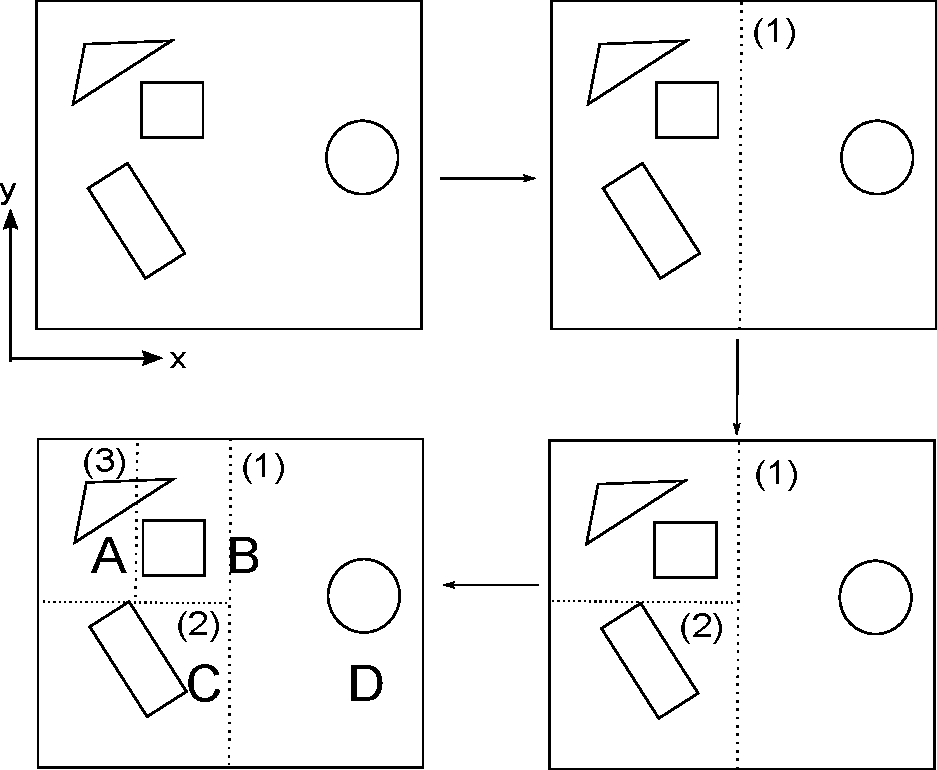
\includegraphics{figKDTreeSubdivideSpatialMid.pdf}} 
    \renewcommand{\thefigure}{\thechapter.\arabic{figure}}
    \caption[The scene with the spatial median subdivision]{\emph{ The scene with the spatial median subdivision}}
    \label{fig:kd-tree_construction_parallel_pattern}
\end{figure}
\end{comment}

\subsubsection{Memory Management}

% Memory access pattern, sequential vs random

% Locality, random access is not cache friendly

% Conventional kd-tree construction algorithm is slow due to the random ram access pattern



